\section{Conditional Directional Fast Path}

\paragraph{Why the intervention rule must change.}
The original ABER cap is maximal under the bearing-independent A1 envelope
proved in the main paper.  Raising that cap by threshold tuning would discard
the premise that makes the cap safe.  We therefore study ABER-FP, a
conditional extension that credits a favorable turn only when a stronger
executed-transition certificate is available, and otherwise returns the
unchanged ABER action.

\paragraph{Directional transition contract.}
For candidate action $u$, let $\Gamma(x,u)$ be a sound tube containing the
complete realized position trace over the next hold interval, let
$\bar s^+(x,u)$ upper-bound the next translational speed, and let
$\underline d_i^+(x,u)$ lower-bound endpoint clearance to obstacle $i$.
ABER-FP accepts $u$ only if
\begin{align}
 \min_{y\in\Gamma(x,u)}\|y-o_i\|-r_i &\ge 0,
 \label{eq:fppath}\\
 \underline d_i^+(x,u)-D(\bar s^+(x,u)) &\ge 0
 \quad\text{for every }i.
 \label{eq:fpend}
\end{align}
Equation~(\ref{eq:fppath}) prevents intersample keepout entry, while
(\ref{eq:fpend}) returns the next sample to the original ABER set
$\mathcal C$.

\paragraph{Complete online algorithm.}
Let $u_{\rm RL}=(f,w)$ after range clipping and first compute
$u_{\rm base}=\operatorname{ABER}(x,u_{\rm RL})$.  Form
\[
 F=f\{1,.75,.5,.25,0\},
\]
\[
 W=\operatorname{unique}\{\operatorname{clip}(w),\
 \operatorname{clip}(w-.5),\
 \operatorname{clip}(w+.5),-1,0,1\}.
\]
The candidate library is
$Q=\operatorname{unique}((F\times W)\cup\{u_{\rm base}\})$, hence
$|Q|\le31$.  Sort $Q$ by increasing
$\|u-u_{\rm RL}\|_2^2$.  Return the first candidate satisfying
(\ref{eq:fppath})--(\ref{eq:fpend}) for every obstacle; if none passes,
return $u_{\rm base}$.  For $m$ obstacles and the fixed library size, the
online work is $O(31m)=O(m)$ and uses no optimization, fitting, interpolation,
or actor update.

\paragraph{Safety composition.}
\textbf{Proposition S1.}  Suppose the original ABER assumptions A1--A2 hold
and the directional contract is sound for every accepted fast-path action.
Starting in $\mathcal C$, ABER-FP has the same sampled and intersample safety
conclusion as ABER.

\emph{Proof.}
If a fast-path candidate is accepted, (\ref{eq:fppath}) keeps its complete
held trace outside every keepout and (\ref{eq:fpend}) places its endpoint in
$\mathcal C$.  If no candidate is accepted, the output is exactly
$u_{\rm base}$, for which the original ABER theorem preserves the same two
properties.  Induction over sample intervals proves the claim. \hfill$\Box$

The proposition is a composition result, not a finite-data guarantee for a
learned tube.  In the deterministic differential-drive benchmark,
$\Gamma(x,u)$ is the exact held line segment and the endpoint is the exact
semi-implicit servo transition, so the premise is exact.  Safety-Gym and
hardware deployment require a separately frozen, held-out accepted path tube;
the current 20 braking traces do not validate this directional premise.
Accordingly, ABER-FP is not enabled in the MuJoCo claims of the main paper.

\begin{table*}[t]
\centering
\small
\setlength{\tabcolsep}{5pt}
\begin{tabular}{llrrrrr}
\toprule
Scene & Method & Collision & Success & Intervention & Recovery/episode
& Success time (s)\\
 & & (\%) & (\%) & step fraction (\%) & & \\
\midrule
Single & ABER    & 0 & 100 & 49.73 & 8.57  & 6.440\\
Single & ABER-FP & 0 & 100 & 23.33 & 0     & 5.265\\
Multi  & ABER    & 0 & 100 & 83.01 & 13.61 & 7.308\\
Multi  & ABER-FP & 0 & 100 & 34.49 & 0     & 6.286\\
\bottomrule
\end{tabular}
\caption{Frozen held-out comparison in the exact differential-drive model.
Each method/scene cell uses 500 non-development seeds.  All 2,000 runs have
zero certificate violations.}
\label{tab:fastpathheldout}
\end{table*}

\begin{figure*}[t]
\centering
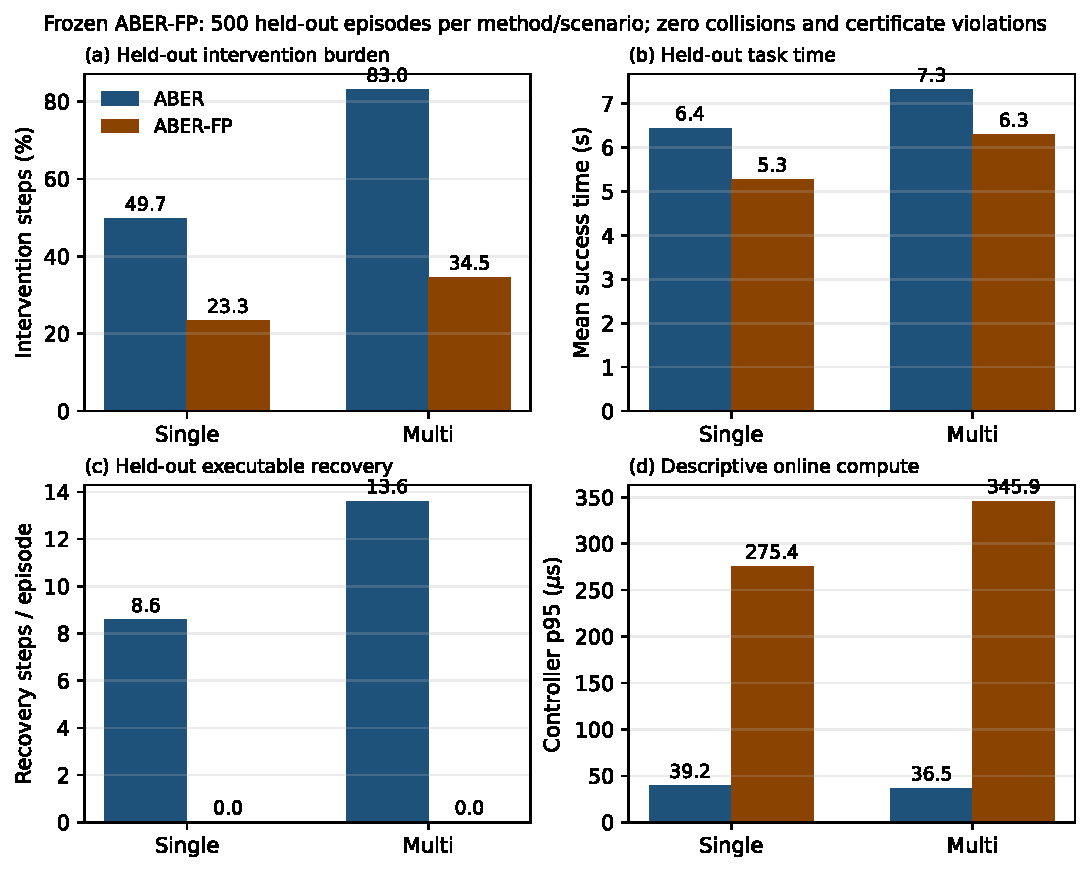
\includegraphics[width=\textwidth]{../figures/supplement/aber_fastpath_performance.pdf}
\caption{Held-out task and intervention performance, with descriptive
controller latency.  ABER-FP lowers intervention occupancy by 53.08\% in the
single-obstacle scene and 58.45\% in the multi-obstacle scene, while reducing
mean success time by 18.24\% and 13.98\%, respectively.}
\label{fig:fastpath}
\end{figure*}

The added check raises controller p95 latency from 39.2 to 275.4~$\mu$s in the
single-obstacle scene and from 36.5 to 345.9~$\mu$s in the multi-obstacle
scene.  The latter is 1.73\% of a 20-ms control period.  These wall times are
machine-specific descriptive measurements; the fixed-library $O(m)$ bound
follows from the implementation.

The executable implementation is
\path{experiments/aaai/aber_fastpath_benchmark.py}; tests are in
\path{tests/test_aber_fastpath.py}.  Frozen development, held-out, and runtime
records are respectively \path{data/aber_fastpath_benchmark.json},
\path{data/aber_fastpath_heldout.json}, and
\path{data/aber_fastpath_runtime.json}.
